
\documentclass[12pt, a4paper]{article}
\usepackage{polski}
\usepackage[utf8]{inputenc}
\usepackage[polish]{babel}
\usepackage{geometry}
\usepackage{hyperref}
\usepackage{amsmath}
\usepackage[numbers]{natbib}
\usepackage{float}
\usepackage{graphicx}
\title{\textbf{Kolaboratywna filtracja na podstawie ocen filmów z bazy MovieLens}}
\author{Marek Lewandowski \\ Michał Karpiuk}
\date{}

\begin{document}
\maketitle

\section{Techniki rekomendacji}
Kolaboratywna filtracja jest jedną z metod implementacji systemów rekomendacji. Inne
dostępne metody to filtracja na podstawie zawartości\footnote{ang. content-based filtering}
oraz techniki hybrydowe, które łączą ze sobą kolaboratywną filtrację z metodami
filtrującymi zawartość. W tej pracy będziemy się posługiwać kolaboratywną filtracją.

\section{Kolaboratywna filtracja}
Algortymy kolaboratywnej filtracji można podzielić na:

\begin{enumerate}
\item oparte na pamięci\footnote{ang. Memory-based algorithms} - w celu predykcji używają całego zbioru danych
\item oparte na modelu\footnote{ang. Model-based algorithms} - w celu predykcji używają
przygotowanego za wczasu modelu
\end{enumerate}

\section{Zadanie}
Naszym zadaniem jest analiza algorytmów kolaboratywnej filtracji. Konkretnie, chcemy
porównać algorytmy UBCF, IBCF i Popular. W tym celu użyjemy języka R, a
dokładnie pakietu ,,Recommenderlab', który zawiera algorytmy kolaboratywnej filtracji i
pozwala na ich ewaluację. 

Będziemy pracować z danymi ze zbioru MovieLens. Używać będziemy danych, które zawierają oceny od 1 do 5 gwiazdek. Od systemów rekomendacji oczekujemy predykcji w podobnej postaci czyli liczonej w gwiazdkach.

\section{Wybrane algorytmy}
Z pakietu ,,Recommenderlab'' wybraliśmy:

\begin{itemize}
\item \textbf{IBCF - Recommender based on item-based collaborative filtering (real data)}\\
Algorytm oparty na modelu (model based), wskazujący rekomendacje przedmiotów na podstawie podobieństwa wybranych i dobrze ocenionych przedmiotów przez użytkownika z innymi przedmiotami.\\
W tym algorytmie wyznaczana jest macierz podobieństwa pomiędzy wszystkimi obiektami w bazie, z czego w celach wydajnościowych, dla każdego obiektu przechowywana jest pewna liczba najpodobniejszych obiektów. Operacja ta powoduje utworzenie modelu, dzięki któremu nie trzeba będzie analizować przy każdej rekomendacji całego zbioru danych.\\
Aby dokonać rekomendacji, analizuje się podobne obiekty, do tych, które aktywny użytkownik ocenił (im lepiej ocenił dany obiekt, tym waga przedmiotów podobnych do niego będzie większa). Po takiej analizie wybierany jest obiekt (lub kilka obiektów), które otrzymały najlepszą ocenę.

\item \textbf{UBCF - Recommender based on user-based collaborative filtering (real data)}\\
Algorytm pamięciowy (memory based), opierający swe działanie na założeniu, że przedmioty wysoko oceniane przez podobnych użytkowników również powinny spodobać się danemu użytkownikowi.\\
W algorytmie tym wyznaczane są współczynniki podobieństw między użytkownikiem aktywnym,\footnote{ang. Active User - użytkownik, dla którego szukamy rekomendacji} a wszystkimi innymi, po czym wybierana jest pewna liczba użytkowników najbardziej podobnych do aktywnego użytkownika. Innym słowem znajdowane jest k-sąsiedztwo użytkownika (k-NN). Następnie na podstawie ocen danego obiektu dokonanych przez k najpodobniejszych użytkowników przewidywana jest ocena obiektu przez aktywnego użytkownika.\\
Za pomocą algorytmu można wyznaczyć ocenę konkretnego obiektu, jak i znaleźć kilka najlepszych rekomendacji dla danego użytkownika.

\item \textbf{POPULAR - Recommender based on item popularity (real data)}\\
Prosty algorytm, który generuje rekomendacje na podstawie popularności obiektów wśród użytkowników.

\end{itemize}


\section{Plan eksperymentów}

\subsection{Pytania badawcze}
Chcemy znaleźć odpowiedzi na następujące pytania:

\begin{enumerate}
\item Jak wyglądają dane z którymi pracujemy? Jak rozkładają się oceny filmów? Jakie mają podstawowe wartości statystyczne?
\item Jak wyglądają dane przed i po ich normalizacji?
\item Który algorytm generuje lepsze wyniki?
\item Który algorytm szybciej generuje wyniki?
\item Jak sposób mierzenia podobieństwa wpływa na wyniki algorytmu?
\item Który z algorytmów ma lepszą skalowalność?
\item Jaki wpływ na wyniki algorytmu ma liczba podobnych użytkowników, używana do predykcji oceny?
\item Jaki wpływ na wyniki algorytmu ma liczba podobnych filmów, używana do predykcji oceny?
\item Który algorytm radzi sobie lepiej dla małej ilości danych?
\item Jak zwiększanie ilości danych wpływa na dokładność algorytmu?
\end{enumerate}

\subsection{Dane}
Skorzystamy ze zbioru co najmniej 100 tysięcy ocen\footnote{w przypadku wystarczającej mocy
obliczeniowej skorzystamy z większej ilości danych} filmów przez użytkowników zawierających
następujace informacje:

\begin{itemize}
\item user id - identyfikator użytkownika
\item item id - identyfikator filmu
\item rating - ocena w skali 1 do 5 gwiazdek
\end{itemize}

Każdy z użytkowników ma co najmniej 20 ocen filmów. Nie przewidujemy potrzeby wcześniejszej obróbki danych.

\subsection{Badane parametry algorytmów}
Będziemy badać następujące parametry:
\begin{itemize}
\item k w kNN \footnote{ang. k-nearest neighbors} - czyli jak ilość podobnych użytkowników / filmów służy predykcji oceny filmu,
\item sposób wyznaczania podobieństwa: cosinus, pearson i inne dostępne miary z pakietu,
\item ilość dostępnych danych.
\end{itemize}


\subsection{Ewaluacja}

\subsubsection{Podział zbioru danych}
Zbiór danych zostanie podzielony na dwa rozłączone podzbiory. Zbiór danych do uczenia się\
\footnote{ang. learning set} oraz zbiór danych testowych\footnote{ang. test set}. Stosunek
zbioru określać będzie parametr $x$, gdzie $x = 0.9$ oznacza, że $90\%$ zbioru danych to
dane do uczenia się, a $10\%$ to dane testowe.

\subsubsection{MAE}
Współczynnik Mean Absolute Error jest popularnym współczynnikiem w ocenie dokładności
algorytmów rekomendacji. Liczy średnią z absolutnej różnicy pomiędzy predykcją, a prawdziwą
oceną.

\begin{math}
MAE = \frac{
        \sum_{\substack{
   \{i, j\}
  }}
  |P_{i,j} - r_{i,j}|
}{n}
\end{math}

\subsubsection{RMSE}
Root Mean Squarred Error (RMSE) jest również używamy do oceny algorytmów. Charakteryzuje
się tym, że bardziej karze większe odchylenia od prawdziwych wartości ocen.

\begin{math}
RMSE = \sqrt{
        \frac{1}{n} \sum_{ \substack{
                \{i,j\}
        } }
        (P_{i,j} - r_{i,j})^2
}
\end{math}
gdzie $n$ to całkowita liczba ocen wszystkich użytkowników. $P_{i,j}$ to predykcja oceny
dla użytkownika $i$ przedmiotu $j$. $r_{i,j}$ to prawdziwa ocena.

\subsubsection{Accuracy}
Określa procent poprawnych rekomendacji, spośród wszystkich dokonanych rekomendacji.\\
$Accuracy = \frac{Poprawne\:rekomendacje}{Wszystkie \:poprawne\: rekomendacje}$
\subsubsection{Precision}
Wskazuje jaka część polecanych obiektów została zarekomendowana poprawnie\\
$Precision = \frac{Poprawne \:rekomendacje}{Wszystkie\: rekomendacje}$
\subsubsection{Recall}
Określa jaki jest procent poprawnych rekomendacji, spośród wszystkich poprawnych rekomendacji wykryto.\\
$Accuracy = \frac{Poprawne\:rekomendacje}{Wszystkie \:możliwe \:poprawne\: rekomendacje}$
\subsubsection{F-Measure}
Wskaźniki Precision i Recall działają antagonistycznie, gdy jeden jest wyższy zazwyczaj wartość drugiego maleje. F-Measure jest złożeniem tych dwóch miar jakości.\\
$F-Measure = \frac{2*Precision*Recall}{Precision + Recall}$


\section{Otwarte kwestie}
Istnieją rozszerzenia dla algorytmów kolaboratywnej filtracji takie jak, domyślne wartości ocen, amplifikacja wag, odwrócona częstość ocen. Jeśli chcielibyśmy sprawdzić jaki wpływ mają takie rozszerzenia na działanie algorytmu musielibyśmy ingerować w kod pakietu ,,Recommenderlab’’. To czy będziemy to robić, jaki jest tego koszt i czy leży to w kwestii naszego zadania pozostaje kwestią otwartą, która będzie można wyjaśnić w momencie, gdy zapoznamy się bliżej z pakietem i jego możliwościami.

Nie wiemy również czy mamy możliwości określenia w jaki sposób ma być budowany model w przypadku IBCF. Z naszej wiedzy wynika, że pakiet Recommenderlab buduje model w oparciu o podobieństwo. Należy sprawdzić czy jest możliwe zbudowanie modelu w oparciu o odchylenia.

\section{Odpowiedzi na pytania badawcze}

\subsection{Jak wyglądają dane z którymi pracujemy? Jak rozkładają się oceny filmów? Jakie mają podstawowe wartości statystyczne?}
Wykres \ref{fig:histogram-ocen-nieznorm} przedstawia rozkład ocen nieznormalizowanych. 

\begin{figure}[H]
  \begin{center}
  \fbox{
    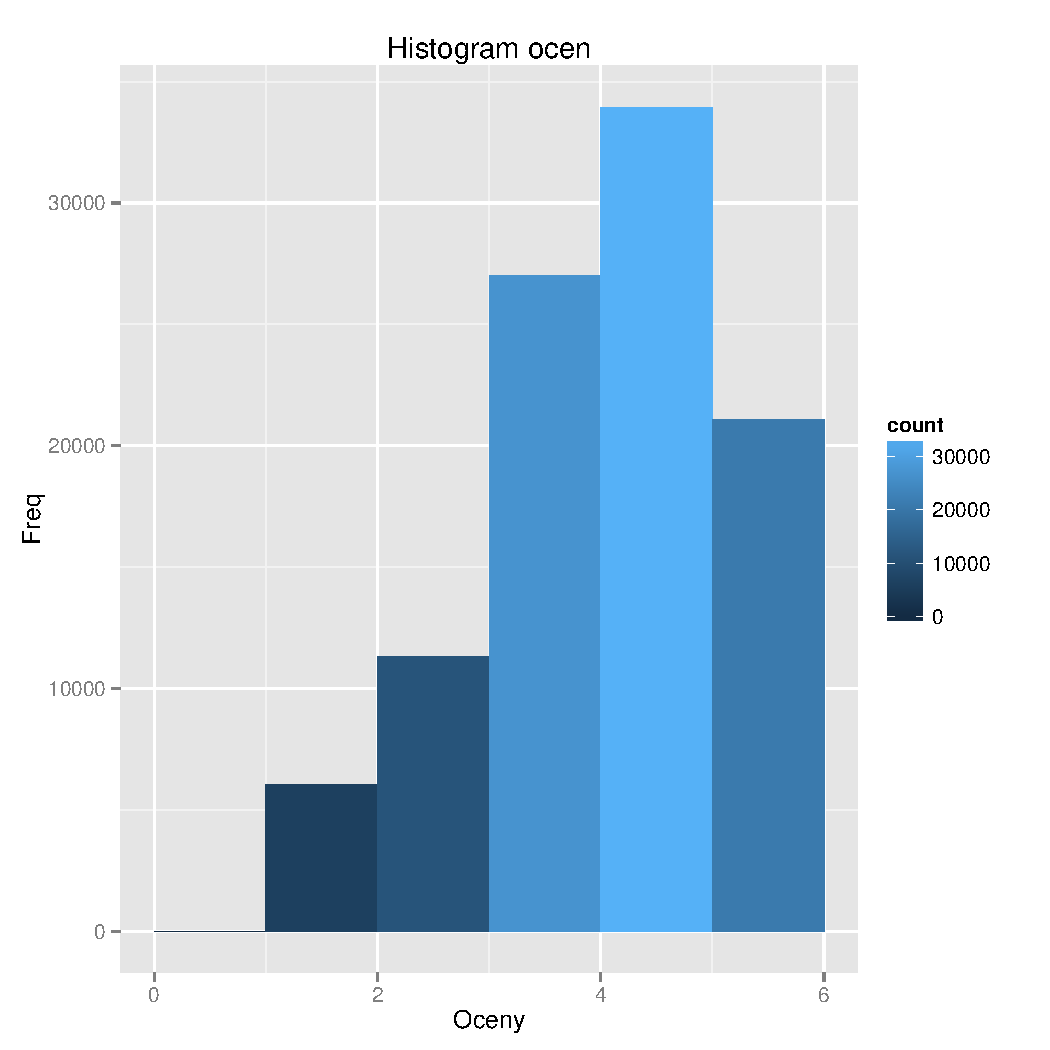
\includegraphics[width=\textwidth]{img/histogram_ocen.pdf}
  }
  \end{center}
  \caption{Rozkład ocen nieznormalizowanych}
  \label{fig:histogram-ocen-nieznorm}
\end{figure}

Poniższa tabelka zawiera statystyki zbioru danych, z którym pracujemy. Statystyki pozwalają zorientować się z tym jak wygląda zbiór danych.
% latex table generated in R 3.0.2 by xtable 1.7-1 package
% Thu Jan 30 21:48:39 2014
\begin{table}[ht]
\centering
\begin{tabular}{rr}
  \hline
 & wartość \\ 
  \hline
Mediana ocen & 4.00 \\ 
  Średnia ocena & 3.53 \\ 
  Najmniejsza liczba ocen & 19.00 \\ 
  Największa liczba ocen & 735.00 \\ 
  Najmniejsza średnia ocena & 1.50 \\ 
  Największa średnia ocena & 4.87 \\ 
  Średnia liczba filmów oceniona przez użytkownika & 105.40 \\ 
   \hline
\end{tabular}
\caption{statystyki zbioru danych} 
\end{table}



\subsubsection{Wnioski}
Patrząc na wykres powyżej, medianę oraz średnią ocene można wywnioskować, że zazwyczaj oceny, które się pojawiają są ocenami pozytywnymi. Oznacza to tyle, że ocenia się częściej to co się lubi i tych ocen jest najwięcej. Dane mogą być jednak zaburzone przez ludzi, którzy oceniają filmy w sposób dla ich tendencyjny np. nie stosując ocen pośrednich dając jedynie oceny najniższe i najwyższe.

\subsection{Jak wyglądają dane przed i po ich normalizacji?}
Wykres \ref{fig:histogram-ocen-norm} przedstawia wyniki znormalizowane. Wyniki nieznormalizowane przedstawione zostały na wykresie \ref{fig:histogram-ocen-nieznorm}. Po normalizacji oceny wyglądają podobnie do rozkładu normalnego.
\begin{figure}[H]
  \begin{center}
  \fbox{
    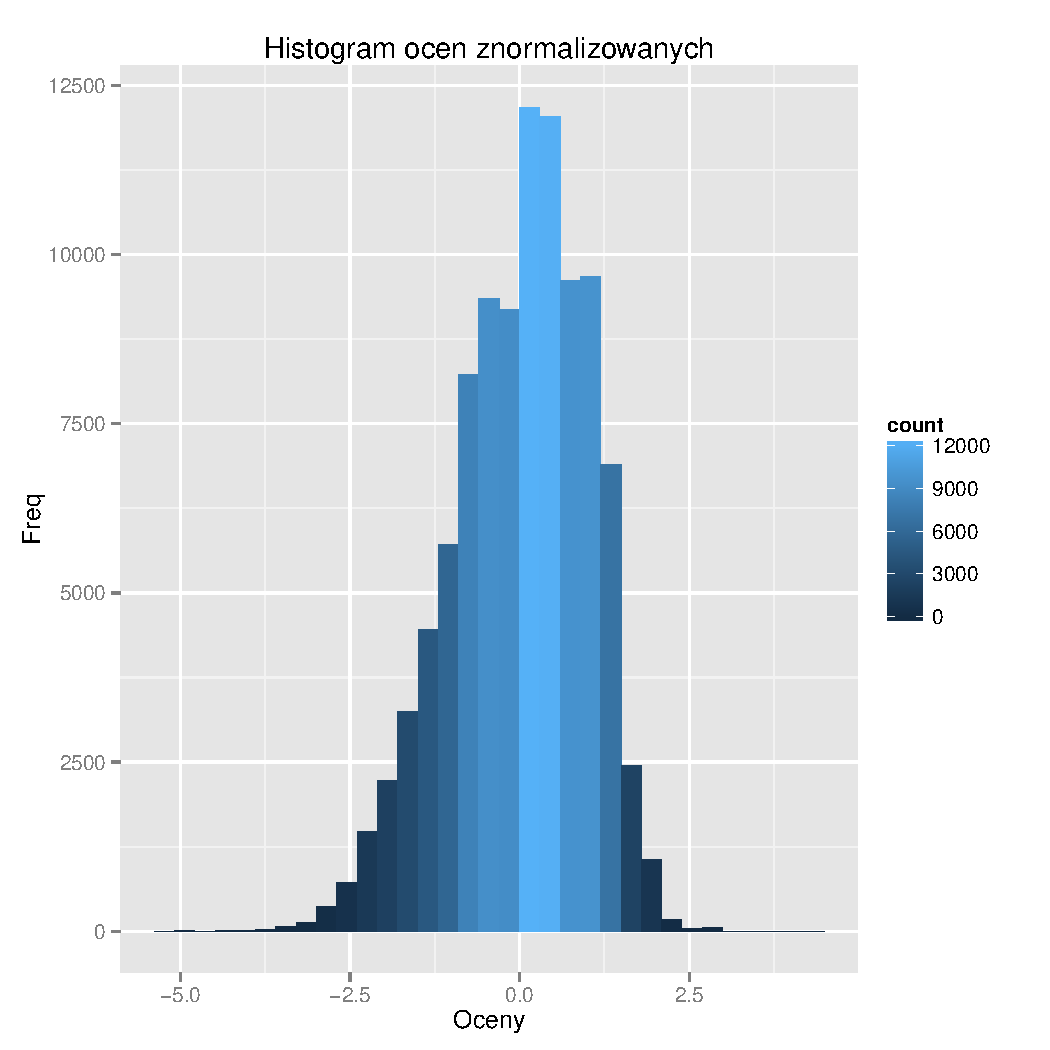
\includegraphics[width=\textwidth]{img/histogram_ocen_norm.pdf}
  }
  \end{center}
  \caption{Rozkład ocen znormalizowanych}
  \label{fig:histogram-ocen-norm}
\end{figure}

\subsubsection{Wnioski}

\subsection{Który algorytm generuje lepsze wyniki?}

\subsubsection{Wnioski}

\subsection{Który algorytm szybciej generuje wyniki?}

\subsubsection{Wnioski}

\subsection{Jak sposób mierzenia podobieństwa wpływa na wyniki algorytmu?}
Sprawdziliśmy w jaki sposób miara podobieństwa użytkowników dla UBCF filmów dla IBCF wpływa na wyniki algorytmu.
Dostępne miary podobieństwa to:
\begin{itemize}
\item Cosinus
\item Pearson
\item Jaccard
\end{itemize}

Różnice w poszczególnych parametrach algorytmów UBCF i IBCF były tylko na poziomie metody obliczania podobieństwa. W ten sposób mogliśmy stwierdzić jak metoda podobieństwa ma wpływ na wyniki algorytmu przy reszcie paramertów takich samych. 

\subsubsection{UBCF}
Wspólne parametry dla algorytmu UBCF:
\begin{itemize}
\item metoda normalizacji: \emph{center}
\item $nn = 25$
\end{itemize}

W przypadku UBCF najlepszą miarą podobieństwa okazał się współczynnik korelacji \emph{Pearson}. Najgorsze wyniki uzyskano dla metody \emph{Jaccard}.

% latex table generated in R 3.0.2 by xtable 1.7-1 package
% Wed Jan 29 19:10:16 2014
\begin{table}[ht]
\centering
\begin{tabular}{rrrr}
  \hline
 & MAE & MSE & RMSE \\ 
  \hline
UBCF cosine & 0.92 & 1.37 & 1.17 \\ 
  UBCF Pearson & 0.92 & 1.39 & 1.18 \\ 
  UBCF Jaccard & 0.93 & 1.39 & 1.18 \\ 
   \hline
\end{tabular}
\caption{Porównanie metod podobieństwa dla UBCF} 
\end{table}



\subsubsection{IBCF}
Wspólne parametry dla algorytmu IBCF:
\begin{itemize}
\item metoda normalizacji: \emph{center}
\item zapamiętana liczba najbardziej podobnych filmów: $k = 30$
% \item $alpha=0.5$ % ta alpha to parametr dla metody liczenia podobieńsa "Karypis" ale my jej nie badamy, bo nie działało 
\end{itemize}

W przypadku IBCF najlepszą miarą podobieństwa okazała się metoda cosinus. W przeciwieństwie do UBCF najgorzej poradził sobie współczynnik korelacji \emph{Pearsona}.

% latex table generated in R 3.0.2 by xtable 1.7-1 package
% Thu Jan 30 12:27:04 2014
\begin{table}[ht]
\centering
\begin{tabular}{rrrr}
  \hline
 & MAE & MSE & RMSE \\ 
  \hline
IBCF cosine & 0.86 & 1.48 & 1.22 \\ 
  IBCF Pearson & 1.16 & 2.11 & 1.45 \\ 
  IBCF Jaccard & 0.90 & 1.54 & 1.24 \\ 
   \hline
\end{tabular}
\caption{Metody podobieństwa dla IBCF} 
\end{table}



\subsubsection{Wnioski}
Na podstawie powyższych badań, można stwierdzić, że nie ma jednej dobrej, uniwersalnej metody badania podobieństwa. Dla algorytmu UBCF właściwym okazał się współczynnik korelacji \emph{Pearsona}, który dla IBCF dawał najgorsze wyniki. Należy zatem dla każdego algorytmu wybrać właściwą dla niego miarę podobieństwa.

\subsection{Który z algorytmów ma lepszą skalowalność?}


\begin{table}[ht]
	\centering
    \begin{tabular}{lll}
    Rozmiar & UBCF & IBCF   \\
    \hline
    188     & 0.02 & 142.10 \\
    376     & 0.02 & 211.10 \\
    564     & 0.03 & 276.39 \\
    752     & 0.03 & 362.03 \\
    940     & 0.03 & 455.23 \\
    \end{tabular}
	\caption{Czas tworzenia modelu w zależności od rozmiaru danych (sekundy)} 
\end{table}
Jak widać... TODO
\begin{table}
	\centering
    \begin{tabular}{lll}
    Rozmiar & UBCF  & IBCF \\
    \hline
    188     & 3.98  & 0.11 \\
    376     & 14.62 & 0.19 \\
    564     & 31.76 & 0.25 \\
    752     & 55.73 & 0.33 \\
    940     & 89.36 & 0.44 \\
    \end{tabular}
    \caption{Czas predykcji w zależności od rozmiaru danych (sekundy)}
\end{table}
\subsubsection{Wnioski}

\subsection{Jaki wpływ na wyniki algorytmu ma liczba podobnych użytkowników, używana do predykcji oceny?}
W tym badaniu interesuje nas parametr $nn$ algorytmu UBCF. 

Parametry algorytmu UBCF podczas badania:
\begin{itemize}
\item metoda normalizacji: \emph{center}
\item miara podobieństwa: \emph{Pearson}
\end{itemize}

Podczas badania zmieniamy wartość parametru $nn$ zaczynając od $nn=30$ aż do $nn=200$ z krokiem $30$. Na początku badaliśmy zmiany $nn$, aż do maksymalnego poziomu - czyli liczby danych, ale dla wysokich wartości parametru $nn$ nie udało się uzyskać wyników, ponieważ błędy były zbyt małymi liczbami. Pakiet \emph{recommenderlab} nie był wstanie wykreślić krzywej ROC, ani \emph{Precision/Recall}.

Poniżej zamieszone zostały wykresy z przeprowadzonych badań. Następnie wyciągnięto z nich wnioski.

\subsubsection{Wartości błędów MAE, MSE, RMSE}
Poniższe wykresy przedstawiają wartości błędów predykcji dla zadanego parametru.

\begin{figure}[H]
  \begin{center}
  \fbox{
    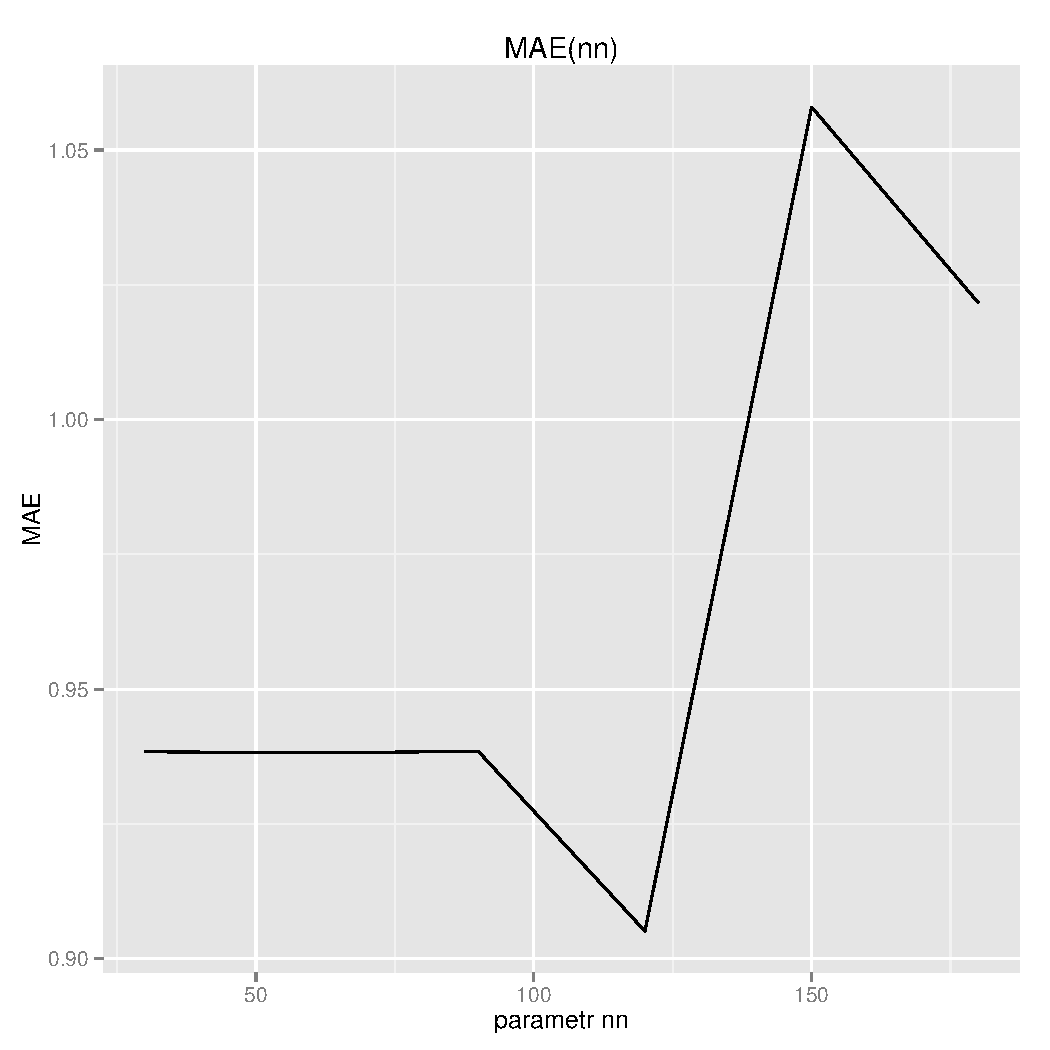
\includegraphics[width=\textwidth, scale=0.5]{img/30-max-50-no-minRating-ubcf-NN-MAE.pdf}
  }
  \end{center}
  \caption{Miara błędu MAE od parametru nn}
  \label{fig:ubcf-nn-mae}
\end{figure}

\begin{figure}[H]
  \begin{center}
  \fbox{
    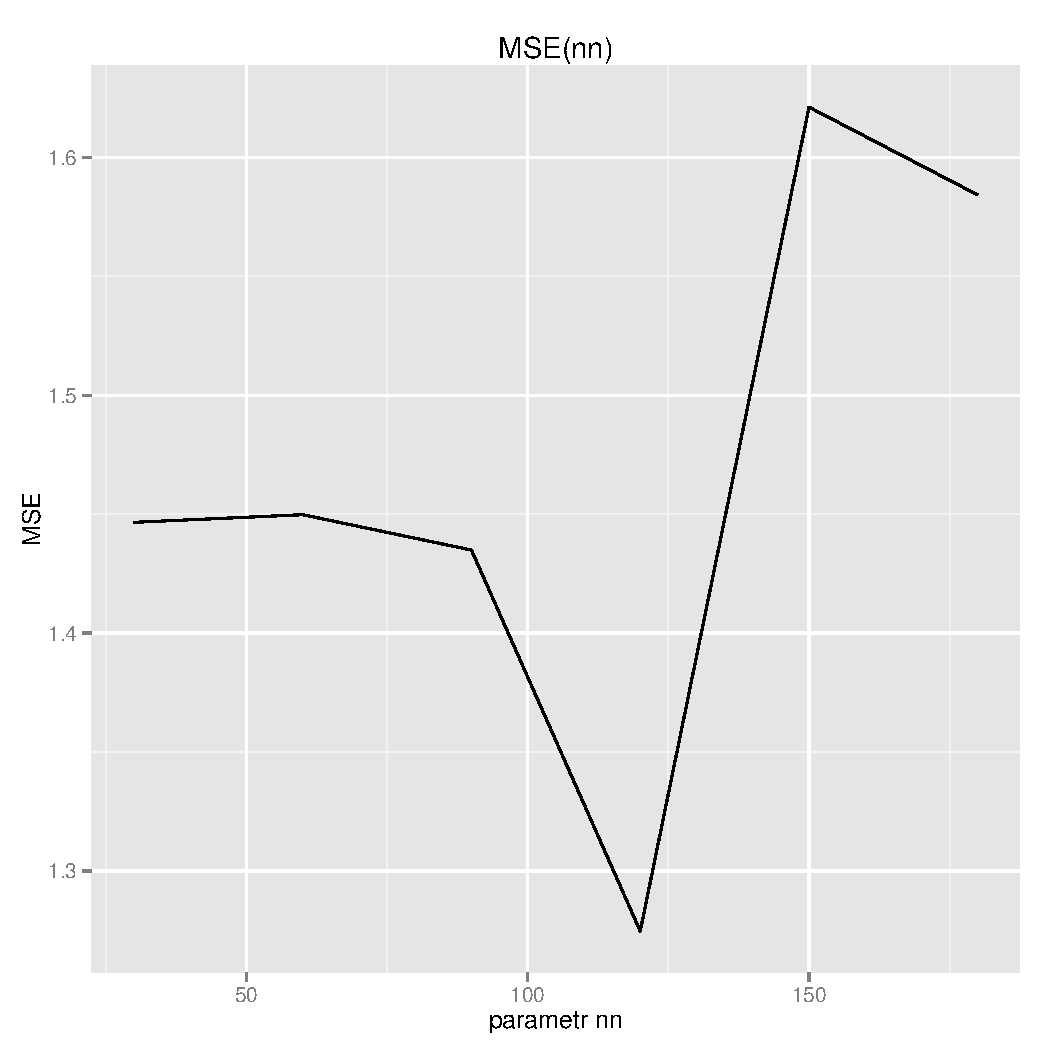
\includegraphics[width=\textwidth, scale=0.5]{img/30-max-50-no-minRating-ubcf-NN-MSE.pdf}
  }
  \end{center}
  \caption{Miara błędu MSE od parametru nn}
  \label{fig:ubcf-nn-mse}
\end{figure}

\begin{figure}[H]
  \begin{center}
  \fbox{
    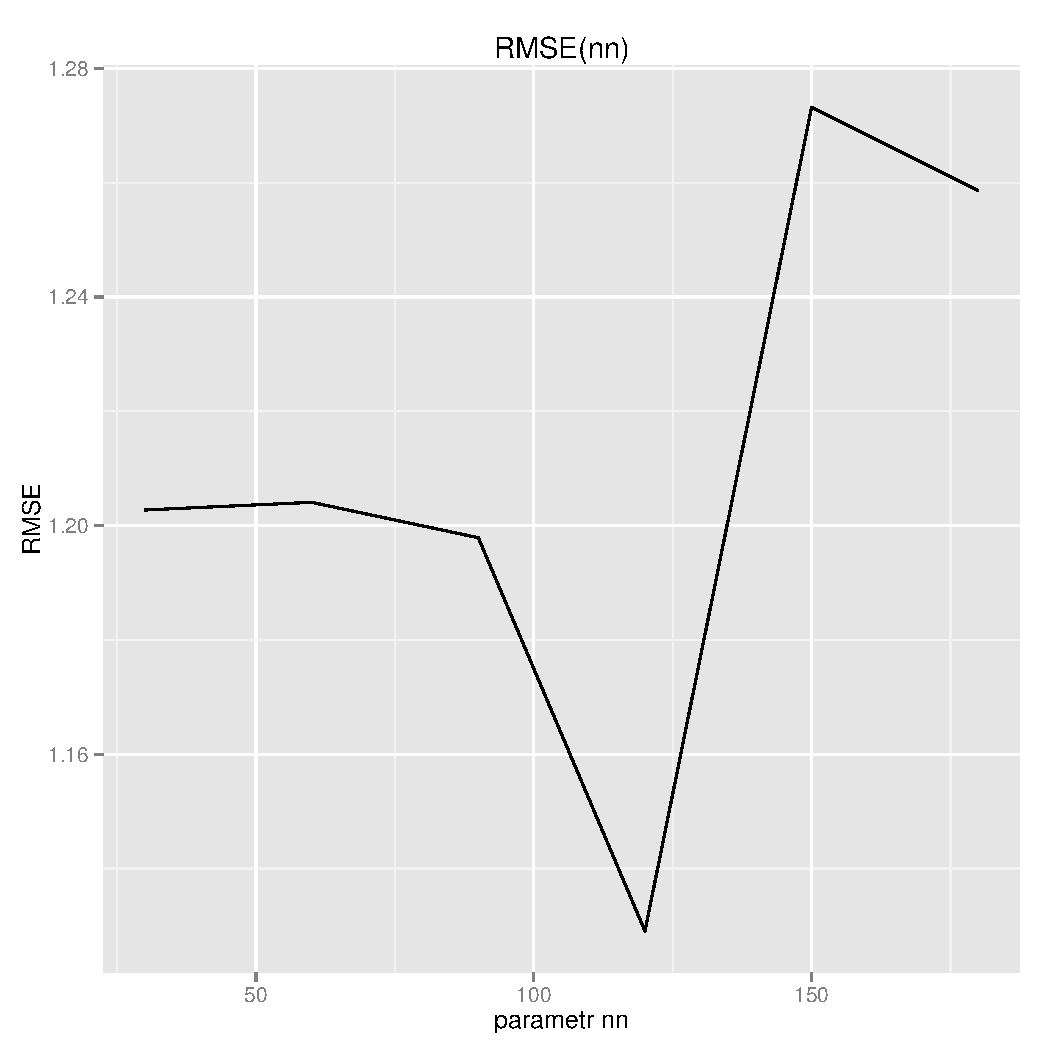
\includegraphics[width=\textwidth, scale=0.5]{img/30-max-50-no-minRating-ubcf-NN-RMSE.pdf}
  }
  \end{center}
  \caption{Miara błędu RMSE od parametru nn}
  \label{fig:ubcf-nn-rmse}
\end{figure}

\subsubsection{Wykres krzywej ROC}

\begin{figure}[H]
  \begin{center}
  \fbox{
    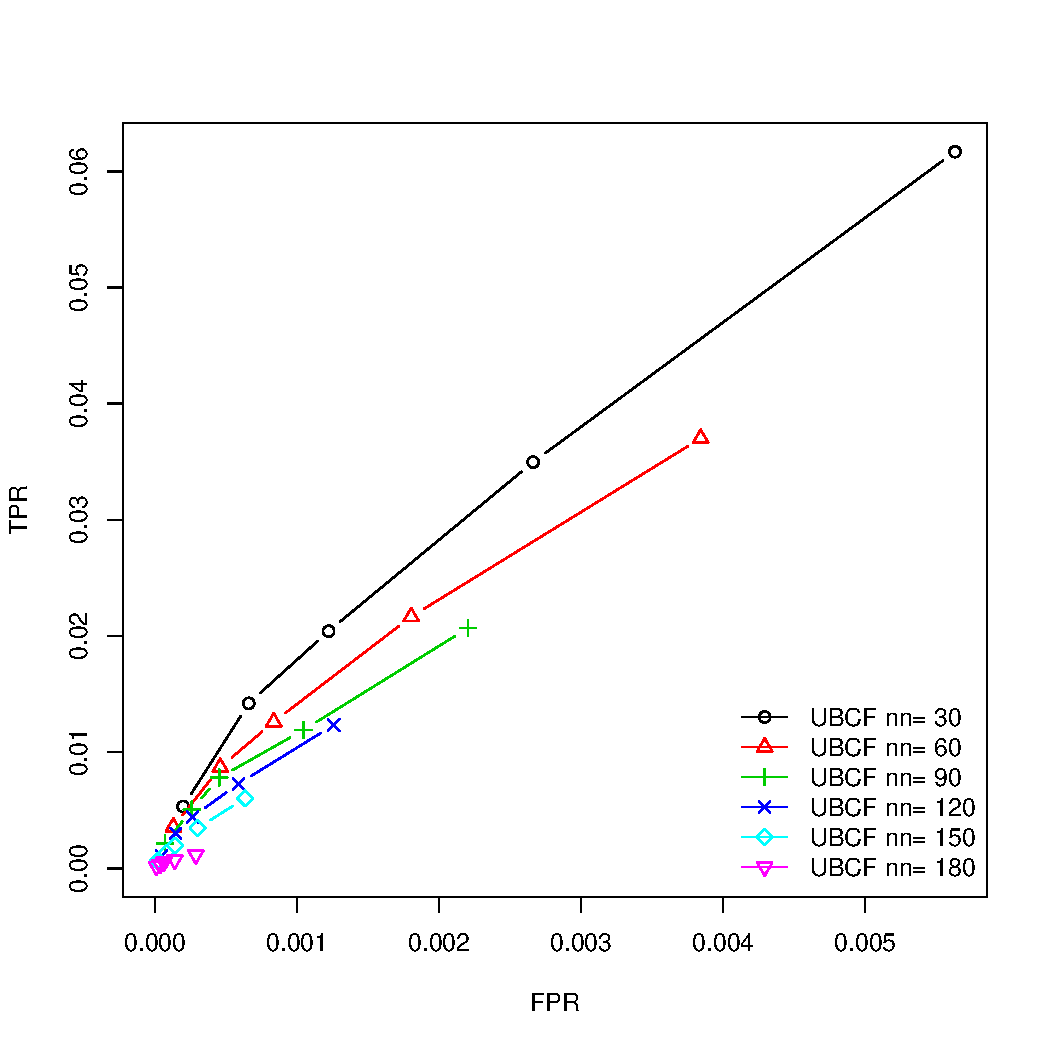
\includegraphics[width=\textwidth, scale=0.5]{img/30-max-50-no-minRating-ubcf-NN-ROC.pdf}
  }
  \end{center}
  \caption{Krzywa ROC w zależności od nn}
  \label{fig:ubcf-nn-rmse}
\end{figure}

\subsubsection{Wykres Precision/Recall}

\begin{figure}[H]
  \begin{center}
  \fbox{
    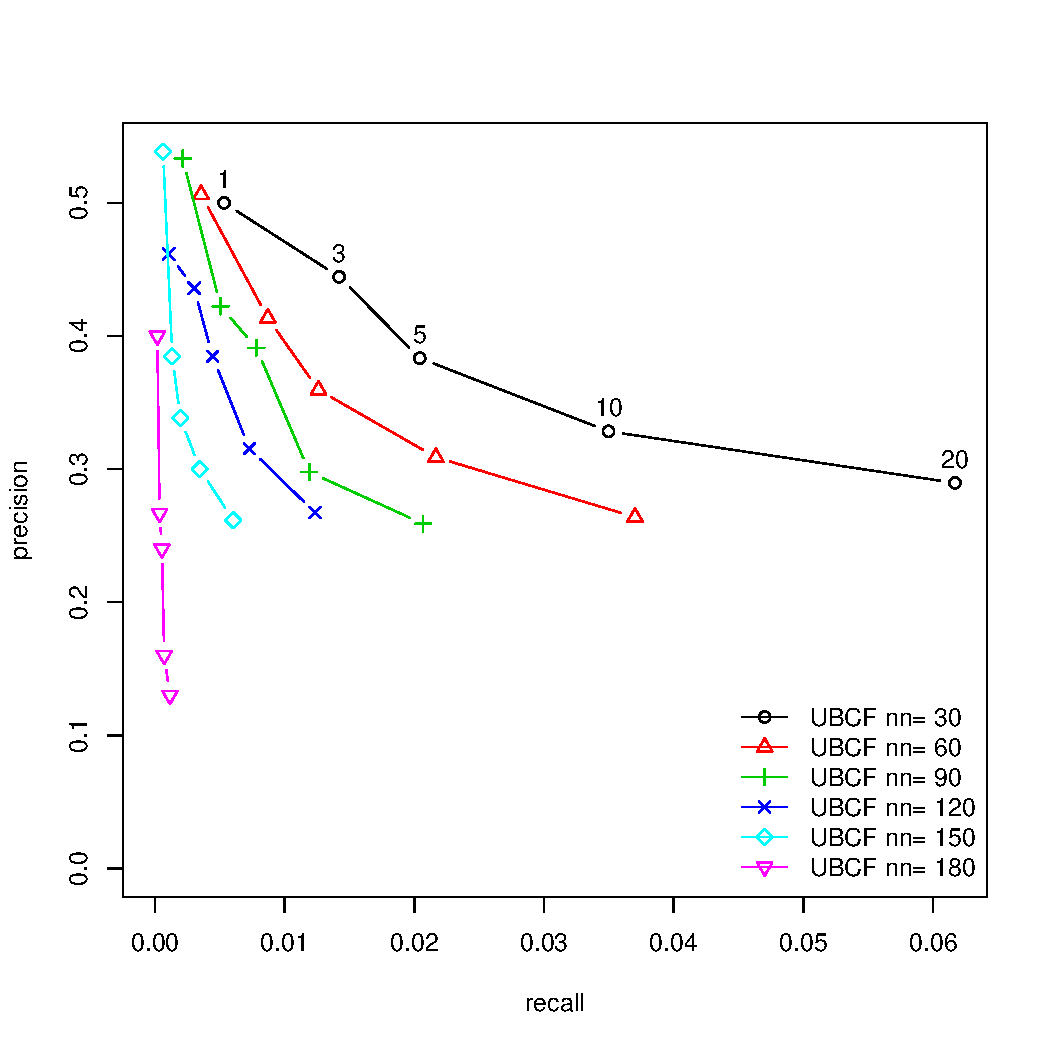
\includegraphics[width=\textwidth, scale=0.5]{img/30-max-50-no-minRating-ubcf-NN-PREC-REC.pdf}
  }
  \end{center}
  \caption{Precision/Recall w zależności od nn}
  \label{fig:ubcf-nn-rmse}
\end{figure}


\subsubsection{Wnioski}
Z wykresów wartości błędów można wywnioskować, że najlepsza wartość parametru znajduje się w okolicy $nn=120$. Dalsze zwiększanie parametru NN - prowadzi do zwiększania się błędów. Można to tłumaczyć tym, że jest to za duża wartość w stosunku do naprawdę innych bliskich osób o podobnych preferencjach. Ze zbyt wysoką wartością $nn$ zaczynamy uwzględniać osoby, które mają odmienne preferencje co prowadzi do gorszych predykcji, a zatem ogólny błąd jest większy.

TODO wnioski na podstawie tego precision recall i ROC

\subsection{Jaki wpływ na wyniki algorytmu ma liczba podobnych filmów, używana do predykcji oceny?}
W tym badaniu interesuje nas parametr $k$ algorytmu IBCF. 

Parametry algorytmu IBCF podczas badania:
\begin{itemize}
\item metoda normalizacji: \emph{center}
\item miara podobieństwa: \emph{Cosinus}
\end{itemize}

Podczas badania zmieniamy parametr k od $k=5$ do $k=150$ ze skokiem $20$. Dla każdego k budujemy model, mierzymy błędy na zbiorze testowym i czasy potrzebne na predykcję i zbudowanie modelu. Następnie porównujemy ze sobą algorytmy z różnymi parametrami $k$.

Wyniki badań przedstawiono na wykresach poniżej. 

\subsubsection{Wartości błędów MAE, MSE, RMSE}
Poniższe wykresy przedstawiają wartości błędów predykcji dla zadanego parametru $k$.

\begin{figure}[H]
  \begin{center}
  \fbox{
    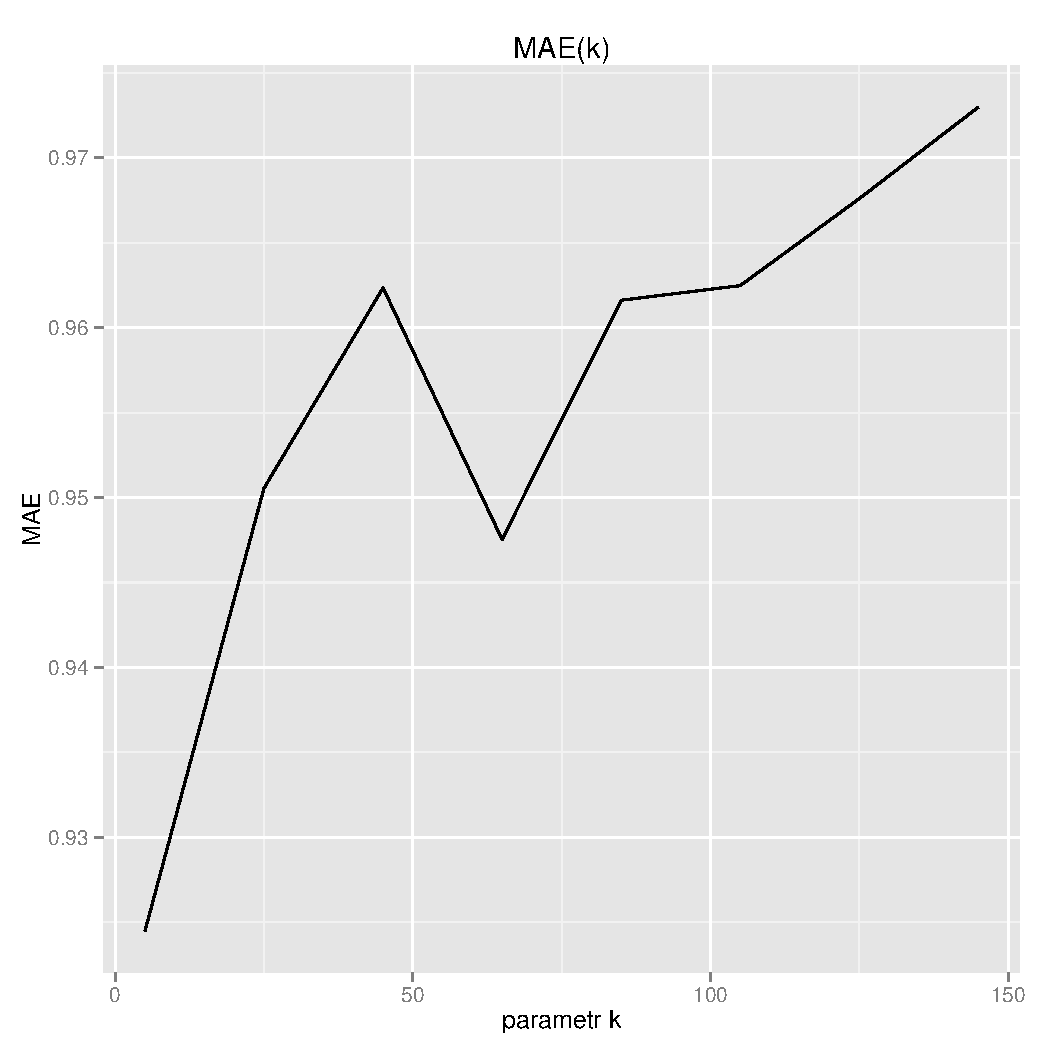
\includegraphics[width=\textwidth, scale=0.5]{img/ibcf-K-MAE.pdf}
  }
  \end{center}
  \caption{Miara błędu MAE od parametru k}
  \label{fig:ibcf-k-mae}
\end{figure}

\begin{figure}[H]
  \begin{center}
  \fbox{
    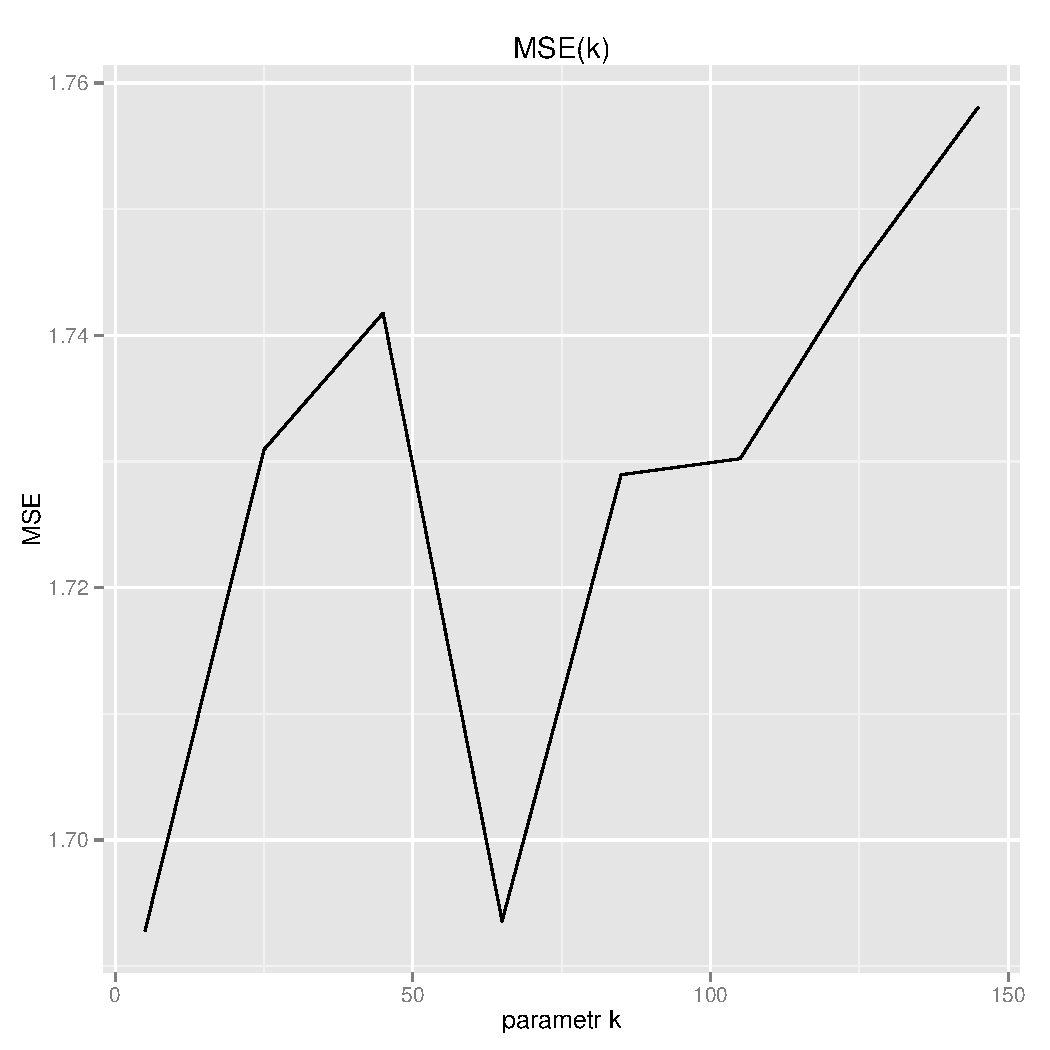
\includegraphics[width=\textwidth, scale=0.5]{img/ibcf-K-MSE.pdf}
  }
  \end{center}
  \caption{Miara błędu MSE od parametru k}
  \label{fig:ibcf-k-mse}
\end{figure}

\begin{figure}[H]
  \begin{center}
  \fbox{
    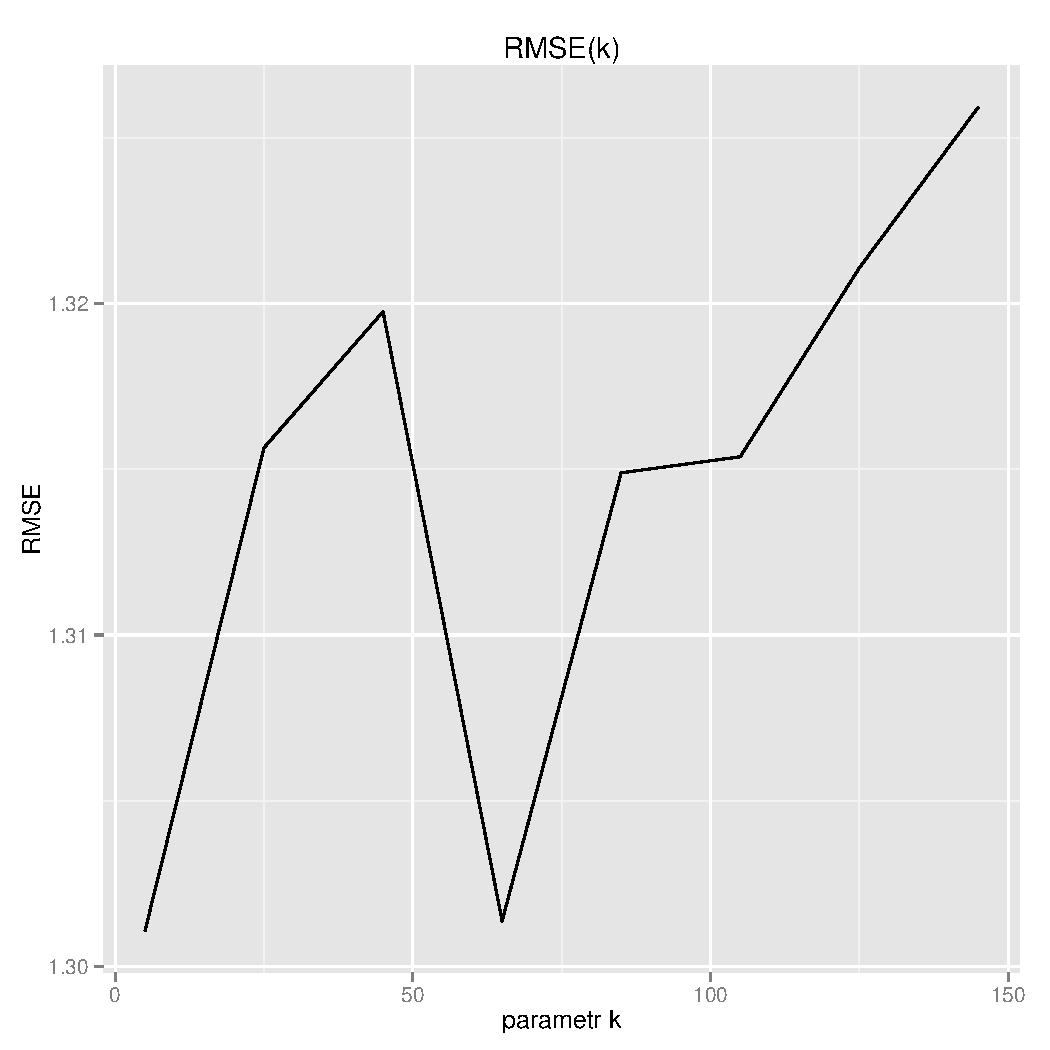
\includegraphics[width=\textwidth, scale=0.5]{img/ibcf-K-RMSE.pdf}
  }
  \end{center}
  \caption{Miara błędu RMSE od parametru k}
  \label{fig:ibcf-k-rmse}
\end{figure}

\subsubsection{Wykres krzywej ROC}

\begin{figure}[H]
  \begin{center}
  \fbox{
    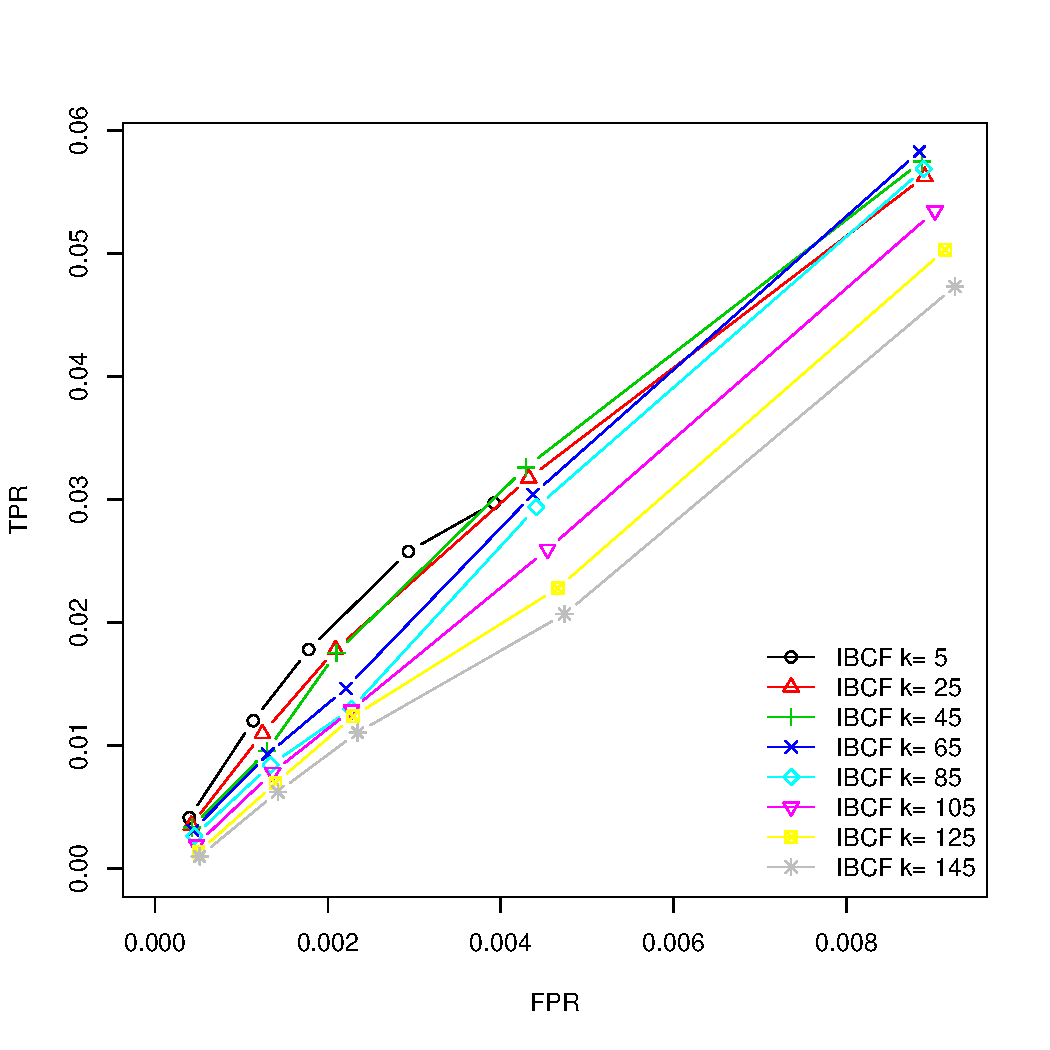
\includegraphics[width=\textwidth, scale=0.5]{img/ibcf-K-ROC.pdf}
  }
  \end{center}
  \caption{Krzywa ROC w zależności od k}
  \label{fig:ibcf-k-roc}
\end{figure}

\subsubsection{Wykres Precision/Recall}

\begin{figure}[H]
  \begin{center}
  \fbox{
    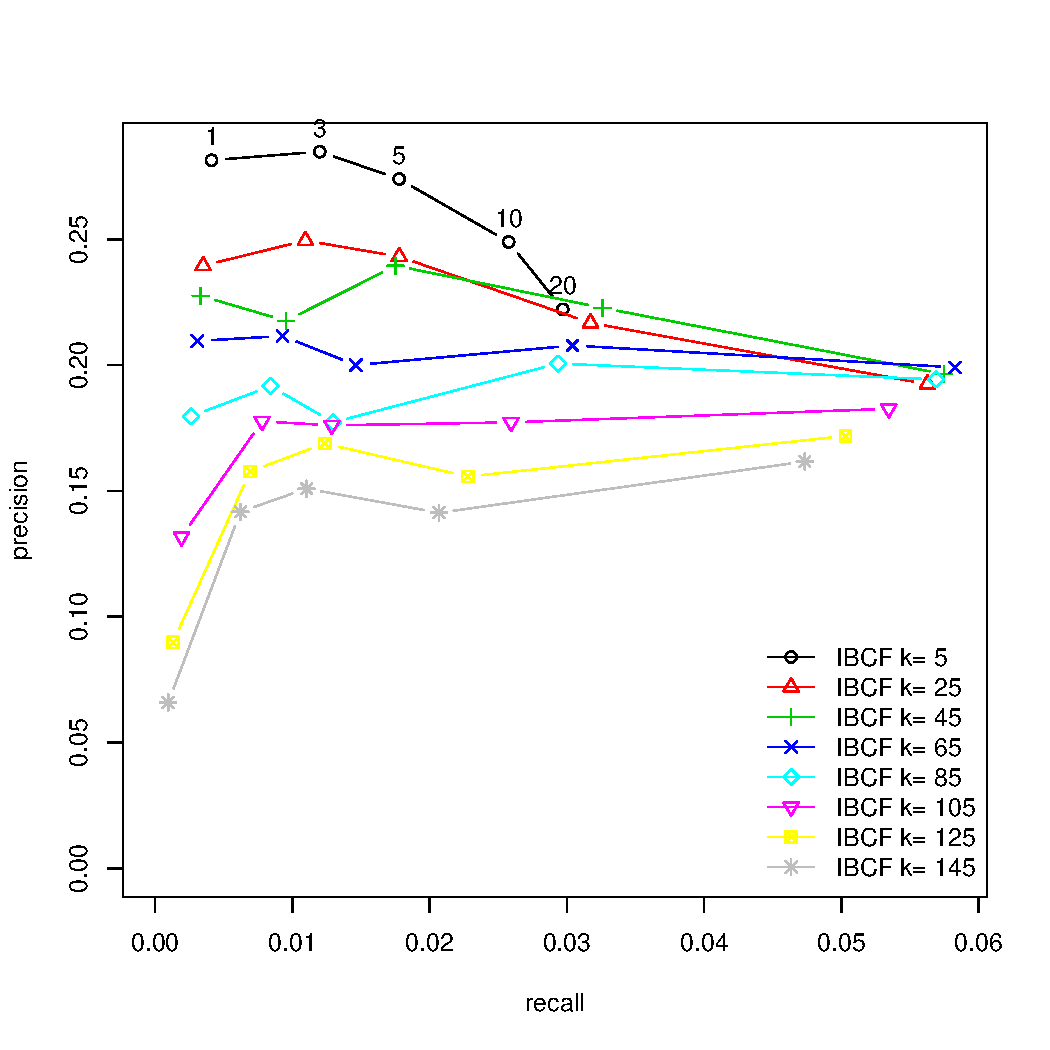
\includegraphics[width=\textwidth, scale=0.5]{img/ibcf-K-PREC-REC.pdf}
  }
  \end{center}
  \caption{Precision/Recall w zależności od k}
  \label{fig:ubcf-nn-rmse}
\end{figure}



\subsubsection{Wnioski}
Analizując wykresy błędów, można dojść do podobnych wniosków jak przy wysokich wartościach parametru $nn$ w algorytmie UBCF - dla dużych wartości $k$ i stosunkowo niedużego zbioru danych zaczynamy brać pod uwagę mało podobne filmy do budowy modelu co przekłada się na gorsze predykcje i większe błędy na zbiorze testowym.

TODO wnioski o ROC, precision/RECALL

\subsection{Który algorytm radzi sobie lepiej dla małej ilości danych?}

\subsubsection{Wnioski}

\subsection{Jak zwiększanie ilości danych wpływa na dokładność algorytmu?}

\subsubsection{Wnioski}

\section{Podsumowanie}

\subsection{Wnioski końcowe}

\nocite{*}
\bibliographystyle{plainnat}
\bibliography{bibliography}
\end{document}

